\documentclass[../momento_1.tex]{subfiles}

\begin{document}

Inicialmente procedi à ativação do agente SNMP na porta 5555. Por defeito, o agente encontra-se configurado para estar à escuta na porta UDP 161 para todas as interfaces IPv4. De forma a fazer esta alteração foi necessário alterar o ficheiro de configuração \textit{snmpd.conf}, como podemos observar na Figura \ref{fig:conf}.\par 

\begin{figure}[H]
\centering
\captionsetup{justification=centering,margin=2cm}
\centerline{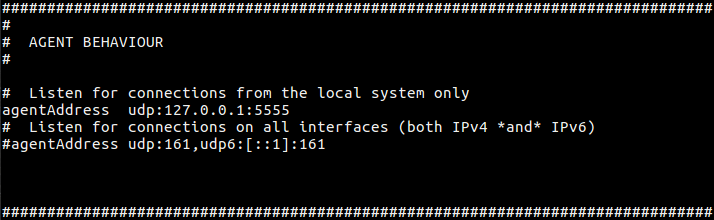
\includegraphics[scale=0.6]{../imagens/port.png}}
\caption{Alteração da porta do agente SNMP.}
\label{fig:conf}
\end{figure}

Após a configuração estar concluída foi possível responder ás questões propostas no enunciado do trabalho prático.\par
 
\textbf{Questão 1 - Qual o valor e significado da instância do objeto com o OID lexicograficamente a
seguir a 1.3.6.1.2.1.6.1 da sua estação de trabalho?}\par

Para conseguir responder a esta questão fiz uso da primitiva \textit{GetNext()} para que fosse possível obter o OID lexicograficamente a seguir a 1.3.6.1.2.1.6.1.
Na Figura \ref{fig:next} podemos ver o comando usado para executar esta operação bem como o resultado obtido.\par

\begin{figure}[H]
\centering
\captionsetup{justification=centering,margin=2cm}
\centerline{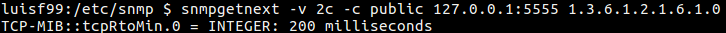
\includegraphics[scale=0.6]{../imagens/getNext.png}}
\caption{Utilização da primitiva \textit{GetNext()}.}
\label{fig:next}
\end{figure}

A resposta a esta questão é então o tcpRtoMin, com o OID .1.3.6.1.2.1.6.2, do tipo \textit{INTEGER32}, que representa o valor mínimo permitido por uma implementação TCP para o tempo limite de retransmissão, medido em milissegundos. Uma semântica mais refinada para objetos deste tipo depende do algoritmo utilizado para determinar o tempo limite de retransmissão, em particular, o algoritmo padrão IETF rfc2988 fornece um valor mínimo. O valor obtido é de 200 milissegundos.\par

\textbf{Questão 2 - Como poderia calcular o número de pacotes IP que ficam num router e já não saem
(i.e., têm esse router como destino final)?}\par

Para calcular o número pretendido para esta questão, pode-se assumir que a resposta assenta na diferença do valor entre dois \textit{object identifier}.
O primeiro é o \textit{ipInReceives} (1.3.6.1.2.1.4.3) que devolve o número total de datagramas que entraram incluindo os que entraram por erro. Já o segundo OID é o \textit{ipForwDatagrams} (1.3.6.1.2.1.4.6.0) que devolve o número de datagramas que entraram mas foram encaminhados para outra entidade ou seja, esta entidade não era o seu destino IP final, como um resultado do qual foi feita uma tentativa de encontrar uma rota para encaminhá-los para esse destino final. Nas Figuras \ref{fig:rec} e \ref{fig:forw} podemos ver os comandos utilizados e respetivos resultados.\par

\begin{figure}[H]
\centering
\captionsetup{justification=centering,margin=2cm}
\centerline{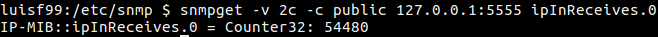
\includegraphics[scale=0.6]{../imagens/ipInReceives.png}}
\caption{Obtenção do valor do \textit{ipInReceives}.}
\label{fig:rec}
\end{figure}

\begin{figure}[H]
\centering
\captionsetup{justification=centering,margin=2cm}
\centerline{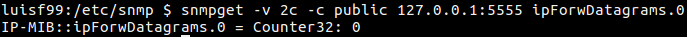
\includegraphics[scale=0.6]{../imagens/ipForwDatagrams.png}}
\caption{Obtenção do valor do \textit{ipForwDatagrams}.}
\label{fig:forw}
\end{figure}

Após a execução destes comandos, podemos afirmar que o resultado final pretendido é de 54480, ou seja, \textit{ipInReceives} - \textit{ipForwDatagrams} = 54480 - 0 = 54480.\par 

\textbf{Questão 3 - Quais as partições do sistema de ficheiros da sua estação de trabalho que a
instrumentação do agente SNMP consegue identificar?}\par

Para responder a esta questão, investiguei o grupo \textit{host} e obtive os valores das instâncias que contém as informações sobre a monitorização do sistema de ficheiros. O \textit{hrStorageTable} lista, em forma de tabela, todo o tipo de dispositivos presentes na máquina, permitindo assim saber as partições do sistema de ficheiros da minha estação de trabalho. Obtive então a resposta a esta questão através do comando ilustrado no Exemplo \ref{lst:comand}, ilustrado na Figura \ref{fig:part}.

{\setstretch{1.1}
\begin{lstlisting}[caption={Comando \textit{hrStorageTable} usado},label={lst:comand},language=JAVA]
	snmptable -v 2c -c public 127.0.0.1:5555 hrStorageTable
\end{lstlisting}}

\begin{figure}[H]
\centering
\captionsetup{justification=centering,margin=2cm}
\centerline{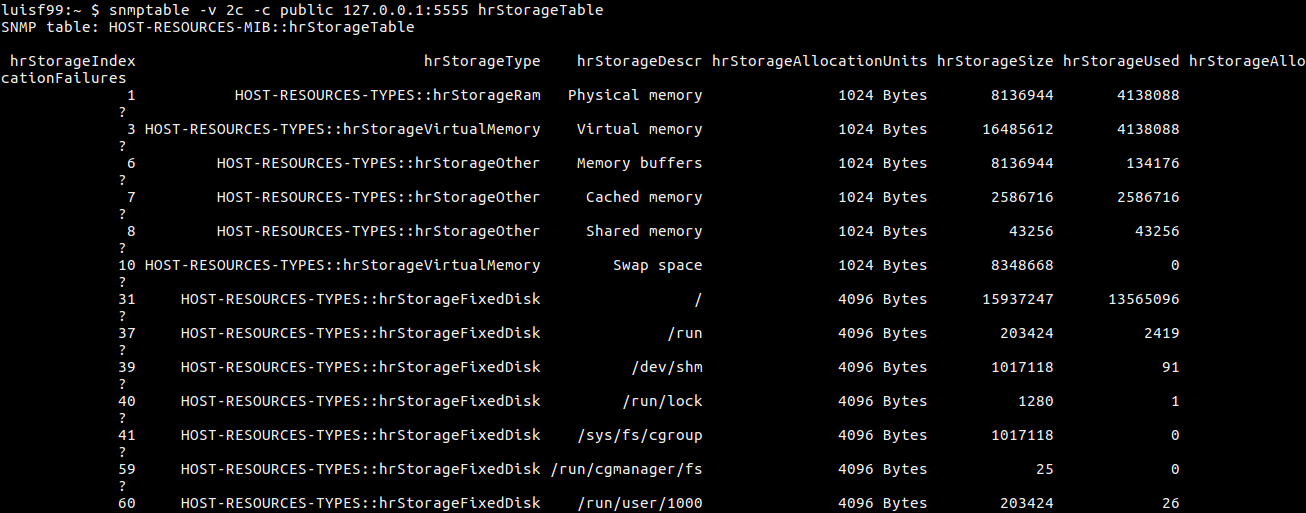
\includegraphics[scale=0.4]{../imagens/storageTable.png}}
\caption{Resultado do comando \textit{hrStorageTable}.}
\label{fig:part}
\end{figure}
\end{document}